\documentclass{estilo}
\usepackage[spanish]{babel}
\usepackage{graphicx}
\usepackage{float}
\usepackage{amsmath}        % para los vectores columnas
\usepackage{amsfonts}       % para las negrita de pizarra
\usepackage{amssymb}        % para simbolos matematicos
\usepackage{multirow}       % para las tablas
\usepackage{dsfont}
\usepackage{listings}
\usepackage{xcolor}
\definecolor{codegreen}{rgb}{0,0.6,0}
\definecolor{codegray}{rgb}{0.5,0.5,0.5}
\definecolor{codepurple}{rgb}{0.58,0,0.82}
\colorlet{backcolour}{uccielo!60}
\lstdefinestyle{mystyle}{
    backgroundcolor=\color{backcolour},
    commentstyle=\color{codegreen},
    keywordstyle=\color{ucazul}\bfseries,
    numberstyle=\tiny\color{codegray},
    stringstyle=\color{codepurple},
    basicstyle=\ttfamily\footnotesize,
    breakatwhitespace=false,
    breaklines=true,
    captionpos=b,
    keepspaces=true,
    numbers=left,
    numbersep=5pt,
    showspaces=false,
    showstringspaces=false,
    showtabs=false,
    tabsize=2
}
\lstset{style=mystyle,
  literate={á}{{\'a}}1 {é}{{\'e}}1 {í}{{\'i}}1 {ó}{{\'o}}1 {ú}{{\'u}}1 {ñ}{{\~n}}1
           {Á}{{\'A}}1 {É}{{\'E}}1 {Í}{{\'I}}1 {Ó}{{\'O}}1 {Ú}{{\'U}}1 {Ñ}{{\~N}}1}


\usepackage{enumitem,multicol,setspace}
\newcounter{subenum}[enumi] % para las multicolumnas
\renewcommand{\thesubenum}{\arabic{subenum}}
\usepackage[nomessages]{fp}
\FPeval\thecolwidth{round(1/4:4)}% Specify number of columns -> column width
\newcommand{\newitem}[1]{%
  \refstepcounter{subenum}%
  \parbox{\dimexpr\thecolwidth\linewidth-.5\columnsep}{%
    \makebox[\labelwidth][r]{(\thesubenum)\hspace*{\labelsep}}%
    #1}\hfill%
}

\usepackage{scalerel,stackengine} % para el sombrero
\stackMath
\newcommand\rhat[1]{%
\savestack{\tmpbox}{\stretchto{%
  \scaleto{%
    \scalerel*[\widthof{\ensuremath{#1}}]{\kern-.6pt\bigwedge\kern-.6pt}%
    {\rule[-\textheight/2]{1ex}{\textheight}}%WIDTH-LIMITED BIG WEDGE
  }{\textheight}%
}{0.5ex}}%
\stackon[1pt]{#1}{\tmpbox}%
}
\parskip 1ex

\usepackage{mathtools}      % floor y ceil
\DeclarePairedDelimiter\ceil{\lceil}{\rceil}
\DeclarePairedDelimiter\floor{\lfloor}{\rfloor}

%% ----------------- Paquetes agregados para este informe -----------------
\usepackage[spanish,ruled,vlined,linesnumbered]{algorithm2e} % pseudocódigo
\usetikzlibrary{babel,arrows.meta,positioning,shapes}          % diagramas
\usepackage{pgfplots}                                          % gráficas teóricas
\pgfplotsset{compat=1.18}
\SetAlCapFnt{\color{ucazul}}            % títulos de algoritmos en azul
\SetAlCapNameFnt{\color{ucazul}}

%% Notación del informe
\newcommand{\N}{\mathbb{N}}
\newcommand{\R}{\mathbb{R}}
\newcommand{\pot}[1]{2^{#1}}                     % conjunto potencia
\newcommand{\MC}{\textsc{Max-Coverage}}
\newcommand{\SC}{\textsc{Set-Cover}}
\newcommand{\SEL}{\textsc{Sel-Sub}}
\newcommand{\REP}{\textsc{Rep-Pres}}
\newcommand{\RED}{\textsc{Red}}


\usepackage[style=authoryear-comp]{biblatex}
\addbibresource{referencias.bib}

%% ----------------- Datos de la portada -----------------
\entrega{Proyecto Semestral 2026-B}
\title{Reparto de presupuesto y\protect\\ selección de participantes}
\subtitulo{Subproyecto 2 --- Análisis de complejidad y NP-dureza (solución base)}
\integrantes{%
  Juan Manuel Martínez Sánchez 46703 \\
  Juan David Reyes Ortiz 54587}
\docente{Luz Enith Guerrero Mendieta}
\date{\today}


\begin{document}
\maketitle

\justifying{}

\newpage
\tableofcontents
\newpage
\section{Introducción}

Una red de $N$ nodos entrena de forma colaborativa un modelo durante varias rondas, sin compartir datos crudos. Cada actualización se protege con ruido calibrado: más ruido protege más, pero reduce la utilidad de la actualización. En cada ronda hay que tomar dos decisiones:
\begin{enumerate}
  \item \textbf{Selección:} qué subconjunto de nodos participa.
  \item \textbf{Reparto:} cuánto del presupuesto de ruido se le asigna a cada nodo seleccionado.
\end{enumerate}

Este informe estudia la dificultad computacional de ambas decisiones. Se demuestra que:
\begin{itemize}
  \item el \textbf{reparto del presupuesto} (Parte 1) se resuelve de forma exacta en tiempo polinomial con un algoritmo voraz, cuya función de eficiencia es $\Theta(N + B\log N)$ en el peor caso;
  \item la \textbf{selección de participantes} (Parte 2) es \textbf{NP-difícil}, mediante una reducción desde \MC{}, de modo que no existe un algoritmo exacto de tiempo polinomial a menos que $\mathrm{P}=\mathrm{NP}$; por ello se usa un algoritmo voraz de aproximación con garantía $(1-1/e)$ y costo $\Theta(N\,k)$ evaluaciones.
\end{itemize}

\section{Preliminares}

\subsection{Notación asintótica}

Sean $T, g : \N \to \R_{\ge 0}$. Se usan las definiciones formales \parencite{cormen2009}:

\begin{definicion}[Cota superior, $O$]
$T(n) \in O(g(n))$ si existen constantes $c > 0$ y $n_0 \in \N$ tales que $T(n) \le c\, g(n)$ para todo $n \ge n_0$.
\end{definicion}

\begin{definicion}[Cota inferior, $\Omega$]
$T(n) \in \Omega(g(n))$ si existen constantes $c > 0$ y $n_0 \in \N$ tales que $T(n) \ge c\, g(n)$ para todo $n \ge n_0$.
\end{definicion}

\begin{definicion}[Cota ajustada, $\Theta$]
$T(n) \in \Theta(g(n))$ si $T(n) \in O(g(n))$ y $T(n) \in \Omega(g(n))$; es decir, existen $c_1, c_2 > 0$ y $n_0$ tales que $c_1 g(n) \le T(n) \le c_2 g(n)$ para todo $n \ge n_0$.
\end{definicion}

\begin{observacion}[Peor caso, mejor caso y cota del algoritmo]\label{obs:casos}
Cuando el número de operaciones depende de los datos (no solo del tamaño), se distinguen $T_{\text{peor}}(n)$ y $T_{\text{mejor}}(n)$. En ese caso se reporta: $T(n)\in O(T_{\text{peor}})$, $T(n)\in\Omega(T_{\text{mejor}})$, y una cota $\Theta$ para cada caso por separado. Cuando el algoritmo realiza siempre las mismas operaciones para un tamaño dado, $T_{\text{peor}} = T_{\text{mejor}}$ y el algoritmo tiene una única cota $\Theta$.
\end{observacion}

\subsection{Modelo de costo}

Se usa el modelo RAM: las operaciones aritméticas, comparaciones, asignaciones y accesos a arreglos cuestan tiempo constante. Para la Parte 2 la utilidad conjunta $f$ se consulta como una función; el costo de una evaluación de $f$ se denota $\tau$ (como en el enunciado) y se reporta por separado, de modo que el costo total se expresa como (número de evaluaciones)$\,\times \tau$.

\subsection{Problemas de decisión, P, NP y reducciones}

Las clases P y NP se definen sobre \textbf{problemas de decisión}, cuya respuesta es \emph{sí} o \emph{no}. Un problema de optimización (``maximizar $f$'') se convierte en uno de decisión agregando un umbral $t$ (``¿existe una solución con valor $\ge t$?'').

\begin{definicion}[Reducción polinomial]
Un problema $A$ se \emph{reduce polinomialmente} a un problema $B$, y se escribe $A \le_p B$, si existe una función $\varphi$, calculable en tiempo polinomial, que transforma cada instancia $I$ de $A$ en una instancia $\varphi(I)$ de $B$ tal que
\[
I \text{ tiene respuesta \emph{sí} en } A \iff \varphi(I) \text{ tiene respuesta \emph{sí} en } B.
\]
\end{definicion}

\begin{definicion}[NP-difícil y NP-completo]
Un problema $B$ es \emph{NP-difícil} si todo problema de NP se reduce polinomialmente a $B$. Es \emph{NP-completo} si además $B \in \mathrm{NP}$.
\end{definicion}

\begin{teorema}[Herramienta de la reducción]\label{teo:herramienta}
Si $A$ es NP-difícil y $A \le_p B$, entonces $B$ es NP-difícil.
\end{teorema}
\begin{proof}
Sea $X \in \mathrm{NP}$. Como $A$ es NP-difícil, existe $\varphi_1$ polinomial con $X \le_p A$. Por hipótesis existe $\varphi_2$ polinomial con $A \le_p B$. La composición $\varphi_2 \circ \varphi_1$ es polinomial (la composición de polinomios es un polinomio) y conserva la respuesta, porque cada transformación la conserva. Así $X \le_p B$ para todo $X\in\mathrm{NP}$.
\end{proof}

\begin{observacion}[Dirección de la reducción]
Para demostrar que \emph{nuestro} problema $B$ es difícil, la reducción va \textbf{desde} un problema $A$ ya conocido como difícil \textbf{hacia} $B$. La interpretación es: si existiera un algoritmo polinomial para $B$, se podría resolver $A$ en tiempo polinomial transformando sus instancias con $\varphi$. Reducir en la dirección contraria ($B \le_p A$) solo mostraría que $B$ \emph{no es más difícil} que $A$, lo cual no aporta nada.
\end{observacion}

\subsection{El conjunto potencia \texorpdfstring{$\pot{V}$}{2\^{}V}}

Para un conjunto finito $V$, $\pot{V}$ denota el \emph{conjunto potencia}: el conjunto de \textbf{todos} los subconjuntos de $V$. Una función de la forma $f:\pot{V}\to\R_{\ge 0}$ recibe un \emph{subconjunto} de $V$ y devuelve un número.

\begin{lema}\label{lem:potencia}
Si $|V| = N$, entonces $|\pot{V}| = 2^N$ y $\displaystyle\sum_{k=0}^{N}\binom{N}{k} = 2^N$.
\end{lema}
\begin{proof}
Para formar un subconjunto, cada uno de los $N$ elementos tiene dos opciones independientes: pertenecer o no pertenecer. Por el principio multiplicativo hay $2\cdot 2\cdots 2 = 2^N$ subconjuntos. Agrupándolos por tamaño, hay exactamente $\binom{N}{k}$ subconjuntos de tamaño $k$, y al sumar sobre $k=0,\dots,N$ se cuenta cada subconjunto una sola vez.
\end{proof}

La Figura~\ref{fig:arbol} muestra los subconjuntos de $V=\{1,2,3\}$ organizados en un árbol: a cada nodo solo se le agregan elementos mayores que su máximo, por lo que ningún subconjunto se repite. El nivel $k$ del árbol contiene los $\binom{3}{k}$ subconjuntos de tamaño $k$, que son exactamente los candidatos del problema de selección con cupo $k$.

\begin{figure}[H]
\centering
\begin{tikzpicture}[
  every node/.style={circle,draw,thick,minimum size=9mm,inner sep=1pt,font=\small},
  level distance=13mm]
  \node (e) at (0,0) {$\emptyset$};
  \node (1) at (2.4, 1.3) {$1$};
  \node (2) at (2.4, 0)   {$2$};
  \node (3) at (2.4,-1.3) {$3$};
  \node (12) at (4.8, 2.0) {$1,2$};
  \node (13) at (4.8, 0.8) {$1,3$};
  \node (23) at (4.8,-0.4) {$2,3$};
  \node (123) at (7.2, 2.0) {\scriptsize $1,2,3$};
  \draw (e)--(1); \draw (e)--(2); \draw (e)--(3);
  \draw (1)--(12); \draw (1)--(13); \draw (2)--(23);
  \draw (12)--(123);
  \begin{scope}[every node/.style={font=\footnotesize}]
    \node at (0,-2.5)   {$\binom{3}{0}=1$};
    \node at (2.4,-2.5) {$\binom{3}{1}=3$};
    \node at (4.8,-2.5) {$\binom{3}{2}=3$};
    \node at (7.2,-2.5) {$\binom{3}{3}=1$};
  \end{scope}
\end{tikzpicture}
\caption{Árbol de los $2^3=8$ subconjuntos de $V=\{1,2,3\}$, agrupados por tamaño.}
\label{fig:arbol}
\end{figure}

\newpage
\section{Formulación matemática de los problemas}

\subsection{Problema 1: reparto óptimo del presupuesto (\REP)}

\begin{definicion}[Reparto óptimo del presupuesto]\label{def:rep}
\textbf{Entrada:} $N$ nodos ya seleccionados para la ronda; para cada nodo $i\in\{1,\dots,N\}$, \textbf{su} función de utilidad $u_i:\N\to\R$, creciente y cóncava; y un presupuesto total $B\in\N$, medido en unidades enteras.

\textbf{Salida:} un reparto $(x_1,\dots,x_N)\in\N^N$, donde $x_i$ es el número de unidades asignadas al nodo $i$.

\textbf{Objetivo:}
\[
\max_{x_1,\dots,x_N}\ \sum_{i=1}^{N} u_i(x_i)
\quad\text{sujeto a}\quad \sum_{i=1}^{N} x_i \le B,\qquad x_i\in\N .
\]
\end{definicion}

\paragraph{Ganancia marginal.} La ganancia de dar la unidad número $x+1$ al nodo $i$ es
\[
g_i(x) = u_i(x+1) - u_i(x), \qquad x = 0,1,2,\dots
\]
\textbf{Creciente} significa $g_i(x)\ge 0$. \textbf{Cóncava} (en el caso discreto) significa que las ganancias no aumentan: $g_i(0) \ge g_i(1) \ge g_i(2) \ge \cdots$. Cada unidad adicional aporta igual o menos que la anterior.

\begin{observacion}[$\le B$ o $=B$]
Como cada $u_i$ es creciente, gastar una unidad sobrante nunca reduce la utilidad. Por lo tanto siempre existe un óptimo que usa exactamente $B$ unidades, y el algoritmo de la Sección~\ref{sec:p1} las reparte todas.
\end{observacion}

\paragraph{Tamaño de la entrada y por qué es la medida adecuada.} El problema crece con dos parámetros:
\begin{itemize}
  \item $N$, el número de nodos: cada nodo agrega una función $u_i$ a la entrada y un candidato más a cada decisión.
  \item $B$, el número de unidades de presupuesto: el voraz toma una decisión por unidad, así que $B$ es el número de pasos.
\end{itemize}
Por eso la función de eficiencia es de dos variables, $T(N,B)$. Se supone que evaluar $u_i(x)$ cuesta tiempo constante, como en la utilidad implementada, $u_i(x)=w_i\ln(1+x)$, donde $w_i>0$ mide la cantidad o calidad de los datos del nodo $i$. Con esta convención, la entrada se describe con $N$ números $w_i$ y el número $B$.

\begin{observacion}[Pseudo-polinomialidad]
$B$ se escribe con solo $\lceil\log_2(B+1)\rceil$ bits, pero el voraz hace $B$ pasos. Su costo es polinomial en el \emph{valor} de $B$ y exponencial en la \emph{longitud} de su representación; es decir, es \textbf{pseudo-polinomial}, el mismo fenómeno de la mochila 0/1. La Sección~\ref{sec:pseudo} lo discute y muestra cómo eliminar la dependencia en $B$.
\end{observacion}
\subsection{Problema 2: selección de participantes (\SEL)}

\begin{definicion}[Selección de participantes]\label{def:sel}

\textbf{Entrada:}

Un conjunto de nodos candidatos $V=\{1,\dots,N\}$; una función de utilidad conjunta
$f:\pot{V}\to\R_{\ge 0}$, que asigna a cada grupo de nodos $A\subseteq V$
su utilidad $f(A)$; y un cupo $k\in\N$ con $k<N$.

\vspace{0.2cm}

\textbf{Salida:}

Un grupo $A\subseteq V$ con $|A|=k$.

\vspace{0.2cm}

\textbf{Objetivo:}

\[
\max_{A\subseteq V}\ f(A)
\quad\text{sujeto a}\quad |A|\le k.
\]

\end{definicion}
Como $f$ es monótona, siempre existe un óptimo con $|A|=k$, de modo que pedir $|A|\le k$ o $|A|=k$ da el mismo valor óptimo.

\paragraph{Propiedades de $f$.} Para $A\subseteq V$ y $j\notin A$ se define la ganancia marginal
\[
\Delta_j(A) = f(A\cup\{j\}) - f(A),
\]
es decir, lo que aporta el nodo $j$ al grupo $A$. Se exige que $f$ sea:
\begin{enumerate}
  \item \textbf{Normalizada:} $f(\emptyset)=0$.
  \item \textbf{Monótona:} $A\subseteq B' \Rightarrow f(A)\le f(B')$; equivalentemente, $\Delta_j(A)\ge 0$.
  \item \textbf{Submodular:} para todo $A\subseteq B'\subseteq V$ y $j\notin B'$,
  \[
  \Delta_j(A) \;\ge\; \Delta_j(B').
  \]
  Agregar un nodo a un grupo pequeño aporta al menos lo que aporta agregarlo a un grupo más grande (rendimientos decrecientes). Se usa $B'$, y no $B$, para no confundir este grupo con el presupuesto.
  \item \textbf{Evaluable en tiempo polinomial:} $f$ se da mediante una descripción compacta que permite calcular $f(A)$ en tiempo polinomial. Se denota $\tau$ el costo de una evaluación.
\end{enumerate}

\begin{observacion}[Por qué la condición 4]
El dominio $\pot{V}$ tiene $2^N$ elementos (Lema~\ref{lem:potencia}). Si $f$ se diera como una tabla con todos sus valores, la entrada tendría tamaño exponencial en $N$, y recorrerla parecería ``lineal'' en el tamaño de la entrada, ocultando la dificultad real. Por ello $f$ se describe de forma compacta.
\end{observacion}

\paragraph{Utilidad implementada.} En la implementación se usa la utilidad de \textbf{cobertura}: hay un universo $U$ de categorías de datos, el nodo $j$ tiene datos de las categorías $S_j\subseteq U$, y
\[
f(A)=\Big|\bigcup_{j\in A}S_j\Big| .
\]
Esta $f$ cumple las condiciones 1--4 (Lema~\ref{lem:valida}). Su descripción compacta son los conjuntos $S_j$.

\paragraph{Tamaño de la entrada y por qué es la medida adecuada.}
\begin{itemize}
  \item $N$, el número de candidatos: determina cuántos grupos existen ($2^N$, o $\binom{N}{k}$ con cupo) y cuántos candidatos revisa el voraz en cada paso.
  \item $k$, el cupo: determina cuántos pasos hace el voraz y el tamaño de los grupos que revisa el exacto.
\end{itemize}
El costo de leer la descripción de $f$ queda dentro de $\tau$. Por eso las funciones de eficiencia se expresan como $T(N,k)$ en número de evaluaciones de $f$, y el tiempo total como $T(N,k)\cdot\tau$. Para la cobertura, con $s=\max_j|S_j|$, la Sección~\ref{sec:voraz} precisa $\tau$: $O(s)$ en el voraz y $O(k\,s)$ en el exacto.

\subsection{Versiones de decisión}

\begin{center}
\begin{tabular}{p{0.2\linewidth}p{0.72\linewidth}}
\toprule
\rowcolor{uccielo} \textbf{Problema} & \textbf{Pregunta (sí/no)} \\
\midrule
\REP & Dados $u_1,\dots,u_N$, $B$ y un umbral $t$: ¿existe un reparto con $\sum_i x_i\le B$ y $\sum_i u_i(x_i)\ge t$? \\
\SEL & Dados $V$, $f$, $k$ y un umbral $t$: ¿existe $A\subseteq V$ con $|A|\le k$ y $f(A)\ge t$? \\
\bottomrule
\end{tabular}
\vspace{0.3cm}

\textit{Nota:} Introducimos el umbral $t$ ya que sirve para convertir un problema de optimización en una pregunta de sí o no.
\end{center}

\subsection{Qué problema es el ``B'' de la reducción}\label{sec:cualB}

El proyecto completo (\RED) combina las dos decisiones: elegir el grupo $A$ con $|A|\le k$ y repartir $B$ entre sus nodos. Las dos partes tienen dificultades muy distintas:

\begin{itemize}
  \item \REP{} está en P (Sección~\ref{sec:p1}). Si se lograra reducir un problema NP-difícil hacia \REP, se tendría un algoritmo polinomial para un problema NP-difícil, lo que implicaría $\mathrm{P}=\mathrm{NP}$. Por lo tanto, \textbf{la reducción no puede ir hacia la Parte 1}.
  \item La dificultad del proyecto está en la \textbf{selección}. La reducción se construye hacia \SEL{} (Sección~\ref{sec:reduccion}).
\end{itemize}

Como \SEL{} es un caso particular de \RED{} (tomando utilidades que no dependen del presupuesto, por ejemplo con $B=0$), cualquier algoritmo para \RED{} resuelve \SEL. En consecuencia, la NP-dureza de \SEL{} se traslada al problema completo del proyecto.

\newpage
\section{Algoritmos y funciones de eficiencia}

\subsection{Parte 1: algoritmo voraz con montículo}\label{sec:p1}

\subsubsection{Algoritmo}

La idea es entregar las $B$ unidades una por una, cada vez al nodo cuya \emph{siguiente} unidad aporta más. Cada nodo $i$ tiene \textbf{una} función de utilidad $u_i$ (son $N$ funciones en total, una por nodo, porque cada nodo tiene datos distintos). La ganancia de la unidad número $x+1$ del nodo $i$ se obtiene con una resta,
\[
g_i(x) = u_i(x+1) - u_i(x),
\]
y se calcula \textbf{solo cuando se necesita}, no se construye una tabla de $N\times B$ ganancias. Un montículo de máximos guarda, para cada nodo, la ganancia de su próxima unidad.

\begin{algorithm}[H]
\caption{\textsc{RepartoVoraz}$(N,\ u,\ B)$}\label{alg:reparto}
\KwIn{$N$ nodos; para cada nodo $i$, \textbf{su} función de utilidad $u_i$ (cóncava y creciente); presupuesto $B\ge 1$}
\KwOut{unidades asignadas a cada nodo, $x_1,\dots,x_N$, con $\sum_i x_i = B$}
\lFor(\tcp*[f]{para cada nodo}){$i\leftarrow 1$ \KwTo $N$}{$x_i \leftarrow 0$ \tcp*[f]{el nodo $i$ empieza sin presupuesto}}
$H \leftarrow$ lista vacía\;
\lFor{$i\leftarrow 1$ \KwTo $N$}{agregar $\big(g_i(0),\, i\big)$ a $H$ \tcp*[f]{1.ª unidad del nodo $i$, con su $u_i$}}
\textsc{Construir-Montículo-Max}$(H)$ \tcp*{$O(N)$}
\For{$b\leftarrow 1$ \KwTo $B$}{
  $(g,\,i) \leftarrow$ \textsc{Extraer-Máximo}$(H)$ \tcp*{nodo con mayor ganancia, $O(\log N)$}
  $x_i \leftarrow x_i + 1$ \tcp*{se le da una unidad}
  \textsc{Insertar}$\big(H,\ (g_i(x_i),\, i)\big)$ \tcp*{solo la siguiente ganancia de $i$, $O(\log N)$}
}
\Return{$(x_1,\dots,x_N)$}\;
\end{algorithm}

\paragraph{Correspondencia con la implementación.}
Cada línea del pseudocódigo corresponde a una instrucción de la función \texttt{reparto\_voraz}, que está en el archivo \texttt{code/algoritmos.py}:

\begin{center}
\begin{tabular}{cl}
\toprule
\rowcolor{uccielo} \textbf{Línea} & \textbf{Python} \\
\midrule
1 & \texttt{x = [0] * N} \\
2--3 & \texttt{H = [(-g(i, 0), i) for i in range(N)]} \\
4 & \texttt{heapq.heapify(H)} \\
5 & \texttt{for \_ in range(B):} \\
6 & \texttt{\_, i = heapq.heappop(H)} \\
7 & \texttt{x[i] += 1} \\
8 & \texttt{heapq.heappush(H, (-g(i, x[i]), i))} \\
\bottomrule
\end{tabular}
\end{center}

Como \texttt{heapq} es un montículo de \emph{mínimos}, las ganancias se guardan con signo negativo: la mayor ganancia queda como el número más pequeño y sale primero.

\subsubsection{Optimalidad (argumento de intercambio)}

\begin{teorema}\label{teo:optimo}
El reparto $x^g$ producido por el Algoritmo~\ref{alg:reparto} es óptimo.
\end{teorema}
\begin{proof}
\textbf{Paso 1: la utilidad se escribe como suma de ganancias.} Para cualquier reparto $x$,
\[
\sum_{i=1}^N u_i(x_i) \;=\; \sum_{i=1}^N u_i(0) \;+\; \sum_{i=1}^{N}\sum_{y=0}^{x_i-1} g_i(y),
\]
por suma telescópica. El primer término no depende del reparto, así que maximizar la utilidad equivale a maximizar la suma de las $B$ ganancias marginales usadas.

\textbf{Paso 2: el voraz toma las $B$ mayores ganancias.} En cada iteración el montículo contiene la próxima ganancia de cada nodo, y por concavidad esa es la mayor ganancia aún disponible de ese nodo. Por lo tanto el voraz toma, en cada paso, la mayor ganancia disponible entre todas. \textbf{Sea $\lambda$ la menor ganancia que tomó el voraz}. Entonces toda ganancia tomada es $\ge\lambda$, y toda ganancia no tomada es $\le\lambda$.

\textbf{Paso 3: intercambio.} Sea $x^*$ un reparto óptimo con $x^*\ne x^g$. Por la observación que sigue a la Definición~\ref{def:rep}, se puede tomar $x^*$ con $\sum_i x^*_i=B$, igual que el voraz. Como ambos suman $B$, existen nodos $i$ y $j$ con $x^*_i > x^g_i$ y $x^*_j < x^g_j$. Se construye $x'$ moviendo una unidad de $i$ a $j$ en $x^*$. El cambio en la utilidad es
\[
\underbrace{g_j(x^*_j)}_{\text{unidad que el voraz sí tomó}} \;-\; \underbrace{g_i(x^*_i-1)}_{\text{unidad que el voraz no tomó}} \;\ge\; \lambda - \lambda \;=\; 0,
\]
porque $x^*_j < x^g_j$ implica que el voraz tomó la unidad $x^*_j$ de $j$, y $x^*_i-1 \ge x^g_i$ implica que no tomó la unidad $x^*_i-1$ de $i$. Así $x'$ también es óptimo y está más cerca de $x^g$ (la distancia $\sum_i |x^*_i-x^g_i|$ baja en $2$).

\textbf{Paso 4: conclusión.} Repitiendo el intercambio un número finito de veces se llega a $x^g$ sin disminuir la utilidad. Por lo tanto $x^g$ tiene utilidad igual a la del óptimo.
\end{proof}

\subsubsection{Función de eficiencia por conteo de operaciones}

Sean $c_1,\dots,c_8>0$ constantes del modelo RAM (se supone que evaluar $u_i$, y por lo tanto $g_i$, cuesta tiempo constante). Un montículo binario con $N$ elementos tiene altura $h=\floor{\log_2 N}$.

\begin{center}
\begin{tabular}{clcc}
\toprule
\rowcolor{uccielo} \textbf{Línea} & \textbf{Operación} & \textbf{Costo por ejecución} & \textbf{Veces} \\
\midrule
1 & inicializar $x_i$ & $c_1$ & $N$ \\
2 & crear la lista & $c_2$ & $1$ \\
3 & calcular $g_i(0)$ y agregarla & $c_3$ & $N$ \\
4 & construir montículo & $\le c_4 N$ (CLRS, cap.~6) & $1$ \\
6 & extraer el máximo & entre $c_6$ y $c_6\,h$ & $B$ \\
7 & incrementar $x_i$ & $c_7$ & $B$ \\
8 & calcular $g_i(x_i)$ e insertar & entre $c_8$ y $c_8\,h$ & $B$ \\
\bottomrule
\end{tabular}
\end{center}

La línea 5 (control del ciclo) se absorbe en las constantes de las líneas 6--8.

\paragraph{Peor caso.} Al extraer y al insertar, el elemento recorre toda la altura del montículo ($h$ niveles):
\[
T_{\text{peor}}(N,B) = c_1N + c_2 + c_3N + c_4N + \sum_{b=1}^{B}\big(c_6\floor{\log_2 N} + c_7 + c_8\floor{\log_2 N}\big)
\]
\[
= (c_1+c_3+c_4)\,N + c_2 + c_7\,B + (c_6+c_8)\,B\floor{\log_2 N}.
\]
Para $N\ge 2$ se cumple $\tfrac12\log_2 N \le \floor{\log_2N}\le\log_2N$, $c_2\le c_2N$ y $B\le B\log_2N$, de modo que con $c_{\min}=\min_i c_i$ y $c_{\max}=\max_i c_i$:
\[
\tfrac{c_{\min}}{2}\,\big(N + B\log_2 N\big) \;\le\; T_{\text{peor}}(N,B) \;\le\; 4\,c_{\max}\big(N + B\log_2 N\big).
\]
\resultado{$T_{\text{peor}}(N,B)\in\Theta(N + B\log N)$}

\paragraph{Mejor caso.} Si los elementos se detienen tras una comparación al extraer y al insertar (por ejemplo, cuando todas las ganancias son iguales):
\[
T_{\text{mejor}}(N,B) = (c_1 + c_3 + c_4')\,N + c_2 + (c_6+c_7+c_8)\,B \;\in\; \Theta(N + B),
\]
donde $0<c_4'\le c_4$ es el costo por elemento de construir el montículo (la construcción siempre recorre los $N$ elementos).

\paragraph{Cotas del algoritmo.} Siguiendo la Observación~\ref{obs:casos}:
\[
T(N,B)\in O(N + B\log N), \qquad T(N,B)\in\Omega(N + B).
\]
Cuando $B\ge N$ (caso usual, más unidades que nodos), $N + B\log N \in \Theta(B\log N)$, que coincide con la cota $O(B\log N)$. En todos los casos el algoritmo es polinomial en $N$ y en el \emph{valor} de $B$; la Sección~\ref{sec:pseudo} precisa qué significa esto.

\subsubsection{Pseudo-polinomialidad y presupuesto continuo}\label{sec:pseudo}

\paragraph{Por qué la cota es pseudo-polinomial.} El tamaño de la entrada en bits es del orden de $N$ (los parámetros $w_i$) más $\lceil\log_2(B+1)\rceil$ (el número $B$). El voraz hace $B$ iteraciones, y $B = 2^{\log_2 B}$: si se duplica el número de \emph{dígitos} de $B$, el tiempo se eleva al cuadrado. Por eso $O(N+B\log N)$ es polinomial en el \emph{valor} de $B$ pero exponencial en la \emph{longitud} de su representación, igual que la programación dinámica $O(nW)$ de la mochila 0/1. En la práctica es eficiente siempre que $B$ sea un número moderado (en el proyecto, las unidades de presupuesto de una ronda).

\paragraph{Cómo quitar la dependencia en $B$ (método del umbral).} La prueba de optimalidad muestra que el voraz toma exactamente las ganancias mayores que un umbral $\lambda$. Para un $\lambda$ dado, el número de unidades del nodo $i$ con ganancia $\ge\lambda$ es
\[
c_i(\lambda)=\big|\{x\ge 0 : g_i(x)\ge\lambda\}\big|,
\]
y como $g_i$ es no creciente, $c_i(\lambda)$ se obtiene con búsqueda binaria sobre $x\in\{0,\dots,B\}$ en $O(\log B)$ evaluaciones. Con una segunda búsqueda binaria sobre $\lambda$ se encuentra el umbral para el que $\sum_i c_i(\lambda)$ alcanza $B$, y las unidades empatadas en $\lambda$ se reparten hasta completar $B$. Si las ganancias son enteras y acotadas por $G$, el costo es $O(N\log B\log G)$, polinomial en el número de bits de la entrada. Esto confirma que \REP{} está en P aun cuando $B$ es muy grande. Para los tamaños del proyecto se usa el voraz con montículo, que es más simple y es el que pide el enunciado.

\paragraph{Presupuesto continuo (nivelación, \emph{water-filling}).} Si $x_i\in\R_{\ge0}$ y las $u_i$ son derivables, cóncavas y crecientes, el problema es convexo y las condiciones de optimalidad (KKT) dicen que existe $\lambda\ge 0$ con
\[
u_i'(x_i)=\lambda \ \text{ si } x_i>0, \qquad u_i'(0)\le\lambda \ \text{ si } x_i=0, \qquad \sum_i x_i = B .
\]
Es la versión continua del umbral: todos los nodos que reciben presupuesto terminan con la \emph{misma} ganancia marginal $\lambda$, como agua que se nivela. Para la utilidad implementada, $u_i(x)=w_i\ln(1+x)$, se tiene $u_i'(x)=w_i/(1+x)$ y por lo tanto
\[
x_i(\lambda)=\max\!\left(0,\ \frac{w_i}{\lambda}-1\right).
\]
Como $\sum_i x_i(\lambda)$ es decreciente en $\lambda$, el nivel se encuentra ordenando los $w_i$ y probando cuántos nodos quedan activos, en $O(N\log N)$, o con búsqueda binaria sobre $\lambda$ en $O(N\log(1/\varepsilon))$ para precisión $\varepsilon$. En el caso continuo el costo ya no depende de $B$, porque no hay unidades que entregar una por una.

\subsection{Parte 2: algoritmo exacto (búsqueda exhaustiva)}\label{sec:exacto}

Como \SEL{} es NP-difícil (Sección~\ref{sec:reduccion}), no se conoce un algoritmo exacto polinomial. El algoritmo exacto natural recorre el árbol de decisiones ``incluir / no incluir'' cada nodo.

\begin{algorithm}[H]
\caption{\textsc{SelecciónExacta}$(V, f, k)$}\label{alg:exacto}
\SetKwFunction{FExacto}{Exacto}
\SetKwProg{Fn}{función}{:}{fin}
\KwIn{nodos $V=\{1,\dots,N\}$; utilidad $f$; cupo $k$}
\KwOut{el mejor grupo $A^*$ con $|A^*|=k$ y su utilidad $v^*=f(A^*)$}
\BlankLine
\Fn{\FExacto{$i,\ A$}}{
  \If(\tcp*[h]{caso 1: el cupo ya está lleno}){$|A| = k$}{
    \Return{$\big(f(A),\ A\big)$}\;
  }
  $\textit{quedan} \leftarrow N - i + 1$ \tcp*{nodos que faltan por decidir}
  $\textit{faltan} \leftarrow k - |A|$ \tcp*{lugares libres en el cupo}
  \If(\tcp*[h]{caso 2: no alcanzan los nodos}){$\textit{quedan} < \textit{faltan}$}{
    \Return{$(-\infty,\ \emptyset)$}\;
  }
  $(v_1, A_1) \leftarrow$ \FExacto{$i+1,\ A\cup\{i\}$} \tcp*{caso 3a: incluir el nodo $i$}
  $(v_2, A_2) \leftarrow$ \FExacto{$i+1,\ A$} \tcp*{caso 3b: no incluir el nodo $i$}
  \eIf{$v_1 \ge v_2$}{
    \Return{$(v_1,\ A_1)$}\;
  }{
    \Return{$(v_2,\ A_2)$}\;
  }
}
\BlankLine
$(v^*, A^*) \leftarrow$ \FExacto{$1,\ \emptyset$} \tcp*{llamada inicial}
\Return{$(v^*, A^*)$}\;
\end{algorithm}

\subsubsection{Recurrencia sin poda: \texorpdfstring{$\Theta(2^N)$}{Theta(2\^{}N)}}

Si se elimina el cupo y se recorren todos los subconjuntos (la recursión llega siempre hasta $i>N$ y evalúa $f$ en cada hoja), cada llamada con $n$ nodos por decidir hace dos llamadas con $n-1$ y trabajo constante $c$:
\[
T(n) = 2\,T(n-1) + c, \qquad T(0) = \tau .
\]
Se resuelve por sustitución (desplegando):
\begin{align*}
T(n) &= 2T(n-1) + c \\
     &= 2\big(2T(n-2)+c\big) + c = 2^2T(n-2) + c(2+1) \\
     &= 2^3T(n-3) + c(2^2+2+1) \\
     &\ \ \vdots \\
     &= 2^jT(n-j) + c\sum_{l=0}^{j-1}2^l = 2^jT(n-j) + c\,(2^j-1).
\end{align*}
Con $j=n$: $T(n) = 2^n \tau + c\,(2^n - 1)$. Por lo tanto
\resultado{$T(N) = (\tau + c)\,2^N - c \;\in\; \Theta\!\left(2^N\right)$ (con $\tau$ constante), o $\Theta(2^N \tau)$ en general.}

\subsubsection{Recurrencia con cupo \texorpdfstring{$k$}{k}: \texorpdfstring{$\binom{N}{k}$}{C(N,k)} evaluaciones}

Sea $L(n,r)$ el número de evaluaciones de $f$ (hojas) cuando quedan $n$ nodos por decidir y faltan $r$ por escoger. De las dos llamadas recursivas (líneas 8 y 9):
\[
L(n,r) = L(n-1,\,r-1) + L(n-1,\,r), \qquad L(n,0)=1,\qquad L(n,r)=0 \ \text{si } r>n .
\]
Es la recurrencia del triángulo de Pascal, cuya solución es $L(n,r)=\binom{n}{r}$ (por inducción, usando $\binom{n}{r}=\binom{n-1}{r-1}+\binom{n-1}{r}$). El algoritmo evalúa $f$ exactamente $\binom{N}{k}$ veces, y como cada llamada interna conduce a alguna hoja y la profundidad es a lo sumo $N$, hay a lo sumo $N\binom{N}{k}$ llamadas internas. Entonces
\[
T_{\text{exacto}}(N,k) \in \Omega\!\left(\binom{N}{k}\tau\right), \qquad T_{\text{exacto}}(N,k) \in O\!\left(\binom{N}{k}(N+\tau)\right),
\]
y el número de evaluaciones es exactamente $\binom{N}{k}$, es decir $\Theta\big(\binom{N}{k}\big)$. El algoritmo hace siempre el mismo recorrido, así que el mejor y el peor caso coinciden.

\subsubsection{Por qué esto no es polinomial}

\begin{lema}\label{lem:binom}
$\displaystyle\binom{N}{\floor{N/2}} \;\ge\; \frac{2^N}{N+1}$.
\end{lema}
\begin{proof}
Por el Lema~\ref{lem:potencia}, los $N+1$ números $\binom{N}{0},\dots,\binom{N}{N}$ suman $2^N$. El mayor de ellos es $\binom{N}{\floor{N/2}}$, y el mayor de $N+1$ números es al menos su promedio, $2^N/(N+1)$.
\end{proof}

Así, para $k=\floor{N/2}$ el algoritmo exacto hace $\Omega(2^N/N)$ evaluaciones: crece de forma \textbf{exponencial}. Para $k$ constante, $\binom{N}{k}\in\Theta(N^k)$, un polinomio cuyo grado crece con $k$; como $k$ es parte de la entrada, el algoritmo no es polinomial en general. Este comportamiento es consistente con la NP-dureza: no se espera que exista un algoritmo exacto polinomial.

\begin{observacion}[Cota del algoritmo vs.\ cota del problema]
Las cotas $O$, $\Omega$ y $\Theta$ anteriores son del \emph{algoritmo exacto}. La NP-dureza no demuestra una cota inferior $\Omega$ exponencial para \emph{todo} algoritmo posible; demuestra que un algoritmo polinomial implicaría $\mathrm{P}=\mathrm{NP}$.
\end{observacion}

\subsection{Parte 2: algoritmo voraz de aproximación}\label{sec:voraz}

\begin{algorithm}[H]
\caption{\textsc{SelecciónVoraz}$(V, f, k)$}\label{alg:voraz}
\KwIn{nodos $V=\{1,\dots,N\}$, utilidad submodular monótona $f$, cupo $k$}
\KwOut{grupo $A$ con $|A| = k$}
$A \leftarrow \emptyset$; $\ f_A \leftarrow 0$ \tcp*{grupo vacío, utilidad $0$}
\For(\tcp*[f]{una vuelta por cada lugar del cupo}){$r\leftarrow 1$ \KwTo $k$}{
  $\textit{mejor}\leftarrow$ ninguno; $\ \textit{mejorDelta}\leftarrow -\infty$\;
  \For{$j\leftarrow 1$ \KwTo $N$}{
    \lIf{$j\in A$}{\textbf{continuar} \tcp*[f]{ya está en el grupo}}
    $\delta \leftarrow f(A\cup\{j\}) - f_A$ \tcp*{$\Delta_j(A)$: una evaluación de $f$}
    \If{$\delta > \textit{mejorDelta}$}{
      $\textit{mejor}\leftarrow j$; $\ \textit{mejorDelta}\leftarrow \delta$\;
    }
  }
  $A \leftarrow A\cup\{\textit{mejor}\}$; $\ f_A \leftarrow f_A + \textit{mejorDelta}$\;
}
\Return{$A$}\;
\end{algorithm}

\paragraph{Correspondencia con la implementación.}\mbox{}\\
En la función \texttt{seleccion\_voraz} del archivo \texttt{code/algoritmos.py} la utilidad es la de cobertura, $f(A)=|C(A)|$. En lugar de guardar $f_A$ se guarda el conjunto \texttt{cubierto} $=C(A)$, y la ganancia de la línea 6 se calcula con el Lema~\ref{lem:ganancia}: \texttt{delta = len(S[j] - cubierto)}, es decir, $\Delta_j(A)=|S_j\setminus C(A)|$. Al agregar el nodo se actualiza \texttt{cubierto |= S[mejor]}.

\paragraph{Conteo de evaluaciones.} En la iteración $i$ quedan $N-(i-1)$ candidatos, y se evalúa $f$ una vez por candidato:
\[
T_{\text{voraz}}(N,k) = \sum_{i=1}^{k}\big(N-i+1\big) = kN - \frac{k(k-1)}{2}.
\]
Como $k<N$, se tiene $\frac{k(k-1)}{2} < \frac{kN}{2}$, y por lo tanto
\[
\frac{kN}{2} \;\le\; T_{\text{voraz}}(N,k) \;\le\; kN .
\]
\resultado{$T_{\text{voraz}}(N,k)\in\Theta(N\,k)$ evaluaciones de $f$; tiempo total $\Theta(N\,k\,\tau)$.}
El algoritmo realiza siempre las mismas iteraciones, así que el mejor y el peor caso coinciden: $O(Nk)$, $\Omega(Nk)$ y $\Theta(Nk)$.

\paragraph{Valor de $\tau$ para la utilidad implementada.} El enunciado exige precisar $\tau$. Con la utilidad de cobertura $f(A)=\big|\bigcup_{i\in A}S_i\big|$ y $s=\max_j|S_j|$:
\begin{itemize}
  \item \textbf{Voraz.} Se mantiene el conjunto de categorías ya cubiertas, $C(A)$, en una tabla hash. Por el Lema~\ref{lem:ganancia}, la ganancia es $\Delta_j(A)=|S_j\setminus C(A)|$, que se calcula recorriendo $S_j$: $\tau=O(s)$. Agregar el nodo elegido a $C(A)$ cuesta otro $O(s)$ por paso. En total,
  \[
  T_{\text{voraz}}(N,k)\in\Theta(N\,k)\ \text{evaluaciones}, \qquad \text{tiempo } O(N\,k\,s).
  \]
  \item \textbf{Exacto.} Cada hoja calcula la unión de $k$ conjuntos desde cero: $\tau=O(k\,s)$. En total, $\binom{N}{k}$ evaluaciones y tiempo $O\big(\binom{N}{k}(N + k\,s)\big)$.
\end{itemize}

\paragraph{Garantía de aproximación.}
\begin{teorema}[\cite{nemhauser1978}]\label{teo:nwf}
Si $f$ es normalizada, monótona y submodular, el grupo $A_g$ del Algoritmo~\ref{alg:voraz} cumple
\[
f(A_g) \;\ge\; \left(1-\frac1e\right) f(A^*) \;\approx\; 0.632\, f(A^*),
\]
donde $A^*$ es un grupo óptimo de tamaño a lo sumo $k$.
\end{teorema}

\textbf{Aplicación.} Las hipótesis del teorema son exactamente las condiciones 1--3 de $f$ en la formulación de \SEL. Para verificarlo en los datos, en instancias pequeñas (donde el Algoritmo~\ref{alg:exacto} es viable) se calcula la razón $f(A_g)/f(A^*)$ y se comprueba que es $\ge 1-1/e$.

\textbf{La cota no se puede mejorar.} \textcite{feige1998} demostró que \MC{} no admite una aproximación mejor que $1-1/e$ en tiempo polinomial a menos que $\mathrm{P}=\mathrm{NP}$. Como \MC{} es un caso particular de \SEL{} (Sección~\ref{sec:reduccion}), el voraz alcanza la mejor garantía posible.

\subsection{Resumen de funciones de eficiencia}

\begin{center}
\renewcommand{\arraystretch}{1.3}
\begin{tabular}{lccc}
\toprule
\rowcolor{uccielo} \textbf{Algoritmo} & $O$ & $\Omega$ & $\Theta$ \\
\midrule
\multirow{2}{*}{Reparto voraz (P1)} & \multirow{2}{*}{$N + B\log N$} & \multirow{2}{*}{$N + B$} & peor: $N + B\log N$ \\
 & & & mejor: $N+B$ \\
\addlinespace
Selección exacta con cupo (P2) & $\binom{N}{k}(N+\tau)$ & $\binom{N}{k}\tau$ & $\binom{N}{k}$ evaluaciones \\
\addlinespace
Selección exacta sin cupo (P2) & $2^N \tau$ & $2^N \tau$ & $2^N \tau$ \\
\addlinespace
Selección voraz (P2) & $NkE$ & $NkE$ & $Nk$ evaluaciones \\
\bottomrule
\end{tabular}
\end{center}

\newpage
\section{NP-dureza de la selección de participantes}\label{sec:reduccion}

La demostración sigue cinco pasos:
\begin{enumerate}
  \item Escoger un problema $A$ conocido como NP-difícil: \MC.
  \item Construir una transformación $\varphi$ desde \MC{} hacia el problema $B=$ \SEL.
  \item Demostrar que $\varphi$ se calcula en tiempo polinomial.
  \item Demostrar que $\varphi$ conserva la respuesta: \emph{sí} en \MC{} $\iff$ \emph{sí} en \SEL.
  \item Concluir que \SEL{} es NP-difícil.
\end{enumerate}

\begin{figure}[H]
\centering
\begin{tikzpicture}[
  caja/.style={draw,thick,rounded corners,align=center,minimum height=12mm,minimum width=33mm,font=\small},
  flecha/.style={-{Stealth[length=3mm]},thick}]
  \node[caja] (sc)  at (0,0)    {\SC\\ \footnotesize NP-completo (Karp)};
  \node[caja] (mc)  at (5,0)    {\MC\\ \footnotesize problema $A$};
  \node[caja,fill=institucionalclaro] (sel) at (10,0) {\SEL\\ \footnotesize problema $B$};
  \draw[flecha] (sc) -- node[above,font=\footnotesize]{$\le_p$} node[below,font=\footnotesize]{Paso 1} (mc);
  \draw[flecha] (mc) -- node[above,font=\footnotesize]{$\le_p$ vía $\varphi$} node[below,font=\footnotesize]{Pasos 2--4} (sel);
\end{tikzpicture}
\caption{Cadena de reducciones. La dificultad se hereda en la dirección de las flechas.}
\end{figure}

%% ---------------------------------------------------------------------
\subsection{Paso 1: problema de partida, Cobertura Máxima}


\begin{definicion}[\MC]
\textbf{Entrada:} $U$, $\mathcal S=\{S_1,\dots,S_m\}$, un entero $k$ y un umbral $t$. \textbf{Pregunta:} ¿existen $k$ conjuntos de $\mathcal S$ cuya unión tiene al menos $t$ elementos?
\end{definicion}

\begin{lema}\label{lem:mc}
\MC{} es NP-completo.
\end{lema}

\textbf{Por qué se escoge \MC.} Su estructura coincide con la de nuestro problema: escoger $k$ elementos (conjuntos o nodos) para maximizar algo en lo que las contribuciones se solapan. Un elemento cubierto por dos conjuntos cuenta una sola vez, igual que la información redundante entre dos nodos.

%% ---------------------------------------------------------------------
\subsection{Paso 2: construcción de la reducción \texorpdfstring{$\varphi$}{phi}}

Dada una instancia $I=(U,\mathcal S=\{S_1,\dots,S_m\},k,t)$ de \MC, se construye la instancia $\varphi(I)=(V,f,k',t')$ de \SEL.

\textbf{Caso trivial $k\ge m$.} \SEL{} exige $k<N$. Si $k\ge m$, en \MC{} se pueden tomar todos los conjuntos y, por monotonía, (con a lo sumo $k$ conjuntos) la respuesta es \emph{sí} exactamente cuando $\big|\bigcup_{i=1}^m S_i\big|\ge t$, lo cual se calcula en tiempo $O(\|I\|)$. En ese caso $\varphi$ devuelve una instancia fija de \SEL{} con la misma respuesta (por ejemplo, $V=\{1,2\}$, $S_1=\{a\}$, $S_2=\emptyset$, $k'=1$ y $t'=1$ para \emph{sí}, o $t'=2$ para \emph{no}). En adelante se supone $k<m$:

\begin{center}
\renewcommand{\arraystretch}{1.3}
\begin{tabular}{p{0.16\linewidth}p{0.27\linewidth}p{0.47\linewidth}}
\toprule
\rowcolor{uccielo} \textbf{Componente} & \textbf{Valor construido} & \textbf{Razón} \\
\midrule
Nodos & $V=\{1,\dots,m\}$, $N=m$ & Cada conjunto $S_i$ se convierte en el nodo $i$; escoger el nodo $i$ equivale a escoger $S_i$. \\
Utilidad & $f(A)=\Big|\bigcup_{i\in A}S_i\Big|$ & La utilidad de un grupo es cuántos elementos distintos cubre: exactamente lo que \MC{} cuenta. \\
Cupo & $k'=k$ & Se escogen tantos nodos como conjuntos. \\
Umbral & $t'=t$ & La utilidad mínima pedida es la cobertura mínima pedida. \\
\bottomrule
\end{tabular}
\end{center}

\textbf{Interpretación en el proyecto.} $U$ son categorías (o regiones) de datos y $S_i$ son las categorías de las que el nodo $i$ tiene datos. La utilidad de entrenar con un grupo es cuántas categorías distintas aporta; una categoría que ya aportó otro nodo no suma de nuevo.

\textbf{Importante:} $V$ son los nodos (lo que se \emph{escoge}) y $U$ son los elementos (lo que se \emph{cubre}).

\begin{algorithm}[H]
\caption{\textsc{Transformar}$(U,\ S_1,\dots,S_m,\ k,\ t)$}\label{alg:tau}
$N\leftarrow m$\;
\For{$i\leftarrow 1$ \KwTo $m$}{
  $\textit{nodo}[i].\textit{conjunto}\leftarrow$ copia de $S_i$\;
}
\Return{$(N,\ \textit{nodo}[1..N],\ k,\ t)$} \tcp*{la descripción de $f$ son los conjuntos}
\end{algorithm}

\begin{algorithm}[H]
\caption{\textsc{Evaluar-}$f(A)$}\label{alg:evalf}
$\textit{cubierto}[1..|U|]\leftarrow \textsc{falso}$; $\ \textit{cont}\leftarrow 0$\;
\ForEach{$i\in A$}{
  \ForEach{$e\in S_i$}{
    \If{\textbf{no} $\textit{cubierto}[e]$}{
      $\textit{cubierto}[e]\leftarrow\textsc{verdadero}$; $\ \textit{cont}\leftarrow\textit{cont}+1$ \tcp*{cada elemento cuenta una vez}
    }
  }
}
\Return{$\textit{cont}$}\;
\end{algorithm}

\subsubsection{La instancia construida es válida}

Para que $\varphi(I)$ sea una instancia de \SEL, $f$ debe cumplir las condiciones de la formulación. Sea $C(A)=\bigcup_{i\in A}S_i$, de modo que $f(A)=|C(A)|$.

\begin{lema}[Ganancia marginal de la cobertura]\label{lem:ganancia}
Para $A\subseteq V$ y $j\notin A$: $\ \Delta_j(A) = |S_j\setminus C(A)|$.
\end{lema}
\begin{proof}
$C(A\cup\{j\}) = C(A)\cup S_j$ es la unión disjunta de $C(A)$ y $S_j\setminus C(A)$. Por lo tanto $f(A\cup\{j\}) = |C(A)| + |S_j\setminus C(A)|$, y al restar $f(A)=|C(A)|$ queda el resultado. En palabras: $j$ aporta solo los elementos que todavía no estaban cubiertos.
\end{proof}

\begin{lema}\label{lem:valida}
La función $f(A)=|C(A)|$ es normalizada, monótona y submodular.
\end{lema}
\begin{proof}
\textbf{Normalizada:} $f(\emptyset)=|\emptyset|=0$.

\textbf{Monótona:} por el Lema~\ref{lem:ganancia}, $\Delta_j(A)=|S_j\setminus C(A)|\ge 0$.

\textbf{Submodular:} sean $A\subseteq B'\subseteq V$ y $j\notin B'$.
\begin{enumerate}
  \item $A\subseteq B'$ implica $C(A)\subseteq C(B')$, porque $B'$ contiene todos los nodos de $A$.
  \item Entonces $S_j\setminus C(B')\subseteq S_j\setminus C(A)$: al quitar un conjunto más grande queda menos.
  \item Por lo tanto $|S_j\setminus C(B')|\le|S_j\setminus C(A)|$.
  \item Por el Lema~\ref{lem:ganancia}, esto es $\Delta_j(B')\le\Delta_j(A)$. \qedhere
\end{enumerate}
\end{proof}

%% ---------------------------------------------------------------------
\subsection{Paso 3: la transformación es polinomial}

Sea $\|I\| = m + |U| + \sum_{i=1}^{m}|S_i|$ el tamaño de la instancia de \MC.

\textbf{Costo de $\varphi$ (Algoritmo~\ref{alg:tau}).} La línea 1 cuesta $c_1$; el ciclo copia cada $S_i$ con costo $c_2|S_i|+c_3$:
\[
T_\varphi(I) = c_1 + \sum_{i=1}^{m}\big(c_2|S_i| + c_3\big) = c_1 + c_3\,m + c_2\sum_{i=1}^{m}|S_i| \;\in\; \Theta\Big(m + \sum_{i}|S_i|\Big)\subseteq O(\|I\|).
\]

\textbf{Costo de evaluar $f$ (Algoritmo~\ref{alg:evalf}).} La inicialización cuesta $\Theta(|U|)$ y el doble ciclo hace $\sum_{i\in A}|S_i|$ iteraciones de costo constante:
\[
\tau(A) \in \Theta\Big(|U| + \sum_{i\in A}|S_i|\Big)\subseteq O(\|I\|).
\]

Ambos costos son \textbf{lineales} en el tamaño de la entrada; en particular, polinomiales. Además, el tamaño de la salida es del mismo orden que el de la entrada, de modo que la instancia construida no crece de forma exponencial.

%% ---------------------------------------------------------------------
\subsection{Paso 4: la transformación conserva la respuesta}

\begin{teorema}\label{teo:conserva}
$I$ tiene respuesta \emph{sí} en \MC{} $\iff$ $\varphi(I)$ tiene respuesta \emph{sí} en \SEL.
\end{teorema}
\begin{proof}
\textbf{($\Rightarrow$)} Supóngase que existen índices $i_1,\dots,i_k$ con $\big|S_{i_1}\cup\dots\cup S_{i_k}\big|\ge t$. Sea $A=\{i_1,\dots,i_k\}$. Entonces $|A|= k$ y
\[
f(A) = \big|S_{i_1}\cup\dots\cup S_{i_k}\big| \ge t,
\]
así que $\varphi(I)$ tiene respuesta \emph{sí}.

\textbf{($\Leftarrow$)} Supóngase que existe $A\subseteq V$ con $|A|\le k$ y $f(A)\ge t$. Los conjuntos $\{S_i : i\in A\}$ son a lo sumo $k$ y su unión tiene $f(A)\ge t$ elementos. Si son menos de $k$, se agregan conjuntos cualesquiera hasta completar $k$ (es posible porque $k<m$); por la monotonía (Lema~\ref{lem:valida}), la unión no disminuye y sigue teniendo al menos $t$ elementos. Por lo tanto $I$ tiene respuesta \emph{sí}.
\end{proof}

\begin{observacion}[Por qué las dos direcciones]
Con solo ($\Rightarrow$), una transformación que siempre produjera instancias con respuesta \emph{sí} pasaría la prueba sin ser una reducción. La dirección ($\Leftarrow$) garantiza que $\varphi$ no crea soluciones que no existían en la instancia original.
\end{observacion}

%% ---------------------------------------------------------------------
\subsection{Paso 5: conclusión}

\begin{teorema}\label{teo:nphard}
\SEL{} es NP-difícil; su versión de decisión es NP-completa.
\end{teorema}
\begin{proof}
Por el Lema~\ref{lem:mc}, \MC{} es NP-difícil. Por los Pasos 2--4, $\varphi$ es una reducción polinomial válida, es decir, $\MC\le_p\SEL$. Por el Teorema~\ref{teo:herramienta}, \SEL{} es NP-difícil. Además, \SEL{} está en NP: un grupo $A$ sirve como certificado, y verificar $|A|\le k$ y $f(A)\ge t$ toma tiempo polinomial porque $f$ es evaluable en tiempo polinomial.
\end{proof}

\begin{corolario}
La versión de optimización de \SEL{}, y por la Sección~\ref{sec:cualB} el problema completo \RED, son NP-difíciles. Si existiera un algoritmo polinomial que encontrara un óptimo $A^*$, bastaría con comparar $f(A^*)\ge t$ para decidir \SEL{} en tiempo polinomial, lo que implicaría $\mathrm{P}=\mathrm{NP}$.
\end{corolario}

\textbf{Consecuencia.} A diferencia de la Parte 1, que se resuelve en $\Theta(N+B\log N)$, para la selección de participantes no se espera un algoritmo exacto polinomial: el exacto conocido hace $\Theta\big(\binom{N}{k}\big)$ evaluaciones, que es exponencial para $k\approx N/2$ (Lema~\ref{lem:binom}). Por eso se usa el voraz de la Sección~\ref{sec:voraz}, con costo $\Theta(Nk)$ y garantía $(1-1/e)$.

%% ---------------------------------------------------------------------
\subsection{Ejemplo de la reducción}

\paragraph{Instancia con respuesta \emph{sí}.} $U=\{1,2,3,4,5,6\}$, $S_1=\{1,2,3\}$, $S_2=\{3,4\}$, $S_3=\{4,5,6\}$, $S_4=\{1,4\}$, $k=2$, $t=6$. Al aplicar $\varphi$: $V=\{1,2,3,4\}$, $f(A)=|C(A)|$, $k=2$, $t=6$.

\begin{center}
\begin{tabular}{cccc}
\toprule
\rowcolor{uccielo} $A$ & $C(A)$ & $f(A)$ & ¿$f(A)\ge 6$? \\
\midrule
$\{1,2\}$ & $\{1,2,3,4\}$ & 4 & no \\
$\{1,3\}$ & $\{1,2,3,4,5,6\}$ & \textbf{6} & \textbf{sí} \\
$\{1,4\}$ & $\{1,2,3,4\}$ & 4 & no \\
$\{2,3\}$ & $\{3,4,5,6\}$ & 4 & no \\
$\{2,4\}$ & $\{1,3,4\}$ & 3 & no \\
$\{3,4\}$ & $\{1,4,5,6\}$ & 4 & no \\
\bottomrule
\end{tabular}
\end{center}

Ambos problemas responden \emph{sí}, con el testigo $A=\{1,3\}$ ($S_1,S_3$).

\paragraph{Submodularidad en números (nodo 2, $S_2=\{3,4\}$).}
\begin{center}
\begin{tabular}{cccc}
\toprule
\rowcolor{uccielo} $A$ & $C(A)$ & $S_2\setminus C(A)$ & $\Delta_2(A)$ \\
\midrule
$\emptyset$ & $\emptyset$ & $\{3,4\}$ & 2 \\
$\{1\}$ & $\{1,2,3\}$ & $\{4\}$ & 1 \\
$\{1,3\}$ & $\{1,\dots,6\}$ & $\emptyset$ & 0 \\
\bottomrule
\end{tabular}
\end{center}

\paragraph{Instancia con respuesta \emph{no}.} Si se cambia $S_3=\{4,5\}$, el elemento $6$ no aparece en ningún conjunto, así que ninguna elección cubre los $6$ elementos: \MC{} responde \emph{no}, y en la instancia construida ningún par alcanza $f(A)=6$, así que \SEL{} también responde \emph{no}.

\newpage
% {\sloppy
% \section{Validación experimental}\label{sec:experimentos}

% \subsection{Metodología}

% \paragraph{Implementación.} Los algoritmos están en \texttt{code/algoritmos.py} y siguen línea a línea los Algoritmos~\ref{alg:reparto}, \ref{alg:exacto} y~\ref{alg:voraz}. Los experimentos están en \texttt{code/experimentos.py}, que genera las tablas (\texttt{code/resultados.json}) y las gráficas (\texttt{img/}). Se ejecutaron con Python 3.13 en un procesador Intel Xeon de 2.8\,GHz.

% \paragraph{Instancias sintéticas (reproducibles).} Todas las instancias se generan con semillas fijas (semilla base $2026$):
% \begin{itemize}
%   \item \textbf{Parte 1.} Pesos $w_i\sim U[1,100]$ y utilidad $u_i(x)=w_i\ln(1+x)$, creciente y cóncava, evaluable en $O(1)$.
%   \item \textbf{Parte 2.} Utilidad de cobertura. Cada nodo $j$ tiene un conjunto $S_j$ de categorías elegidas al azar de un universo $U$, con $|S_j|$ aleatorio entre $s_{\min}$ y $s_{\max}$.
% \end{itemize}

% \paragraph{Medición.} Cada punto es la \textbf{mediana} de 5 ejecuciones (3 para el exacto) medidas con \texttt{time.perf\_counter}, con el recolector de basura desactivado durante la medición, como hace \texttt{timeit}. Se usan entre 6 y 7 tamaños por experimento, duplicando el tamaño en cada paso.

% \paragraph{Contraste con la teoría.} Para cada tamaño se calcula el cociente
% \[
% r = \frac{T_{\text{medido}}}{g},
% \]
% donde $g$ es la función de la cota $\Theta$ deducida. Si la deducción es correcta, $r$ se mantiene aproximadamente constante al crecer el tamaño. En las gráficas, los puntos son los tiempos medidos y la línea es $c\cdot g$, con $c$ igual a la media geométrica de los cocientes $r$ (ajuste por mínimos cuadrados en escala logarítmica). En escala log--log, un costo $n^a$ se ve como una recta de pendiente $a$.

% \subsection{Crecimiento teórico}

% La Figura~\ref{fig:teorico} compara el número de evaluaciones de $f$ que predicen las cotas de la Sección~\ref{sec:exacto} y la Sección~\ref{sec:voraz} con $k=N/2$.

% \begin{figure}[H]
% \centering
% \begin{tikzpicture}
% \begin{semilogyaxis}[
%   width=0.8\linewidth, height=6cm,
%   xlabel={$N$}, ylabel={evaluaciones de $f$},
%   legend pos=north west, legend style={font=\small},
%   grid=major, domain=2:30, samples=29]
%   \addplot[thick,color=red!70!black] {2^x};
%   \addlegendentry{$2^N$ (exacto, todos los subconjuntos)}
%   \addplot[thick,dashed,color=institucional] {x*(x/2)};
%   \addlegendentry{$N\cdot k$ con $k=N/2$ (voraz)}
% \end{semilogyaxis}
% \end{tikzpicture}
% \caption{Crecimiento teórico (escala logarítmica): exponencial frente a polinomial.}
% \label{fig:teorico}
% \end{figure}

% %% ---------------------------------------------------------------------
% \subsection{Parte 1: reparto voraz}

% \paragraph{Optimalidad.} Antes de medir tiempos se comprobó el Teorema~\ref{teo:optimo} contra fuerza bruta: en \textbf{200 instancias} pequeñas ($2\le N\le 4$, $1\le B\le 8$) que enumeran todos los repartos con $\sum_i x_i\le B$, el voraz obtuvo la utilidad óptima en \textbf{200 de 200}.

% \paragraph{Variando $B$ con $N=1000$ fijo.} La teoría predice crecimiento lineal en $B$.

% \begin{table}[H]
% \centering
% \caption{Parte 1 con $N$ fijo. Teoría: $g(N,B)=N+B\log_2 N$.}
% \begin{tabular}{rrrr}
% \toprule
% \rowcolor{uccielo} $N$ & $B$ & $T_{\text{medido}}$ (ms) & $r=T/g$ \\
% \midrule
% 1\,000 & 10\,000 & 7.7 & $7.66\times10^{-8}$ \\
% 1\,000 & 20\,000 & 14.6 & $7.31\times10^{-8}$ \\
% 1\,000 & 40\,000 & 28.8 & $7.20\times10^{-8}$ \\
% 1\,000 & 80\,000 & 59.1 & $7.41\times10^{-8}$ \\
% 1\,000 & 160\,000 & 116.0 & $7.27\times10^{-8}$ \\
% 1\,000 & 320\,000 & 240.2 & $7.53\times10^{-8}$ \\
% \bottomrule
% \end{tabular}
% \end{table}

% \paragraph{Variando $N$ con $B=10N$.} La teoría predice $\Theta(N + B\log N)=\Theta(N\log N)$.

% \begin{table}[H]
% \centering
% \caption{Parte 1 con $B=10N$. Teoría: $g(N,B)=N+B\log_2 N$.}
% \begin{tabular}{rrrr}
% \toprule
% \rowcolor{uccielo} $N$ & $B$ & $T_{\text{medido}}$ (ms) & $r=T/g$ \\
% \midrule
% 1\,000 & 10\,000 & 7.5 & $7.47\times10^{-8}$ \\
% 2\,000 & 20\,000 & 16.0 & $7.24\times10^{-8}$ \\
% 4\,000 & 40\,000 & 34.2 & $7.09\times10^{-8}$ \\
% 8\,000 & 80\,000 & 75.8 & $7.25\times10^{-8}$ \\
% 16\,000 & 160\,000 & 220.2 & $9.79\times10^{-8}$ \\
% 32\,000 & 320\,000 & 582.1 & $1.21\times10^{-7}$ \\
% 64\,000 & 640\,000 & 1547.9 & $1.51\times10^{-7}$ \\
% \bottomrule
% \end{tabular}
% \end{table}

% \begin{figure}[H]
% \centering
% 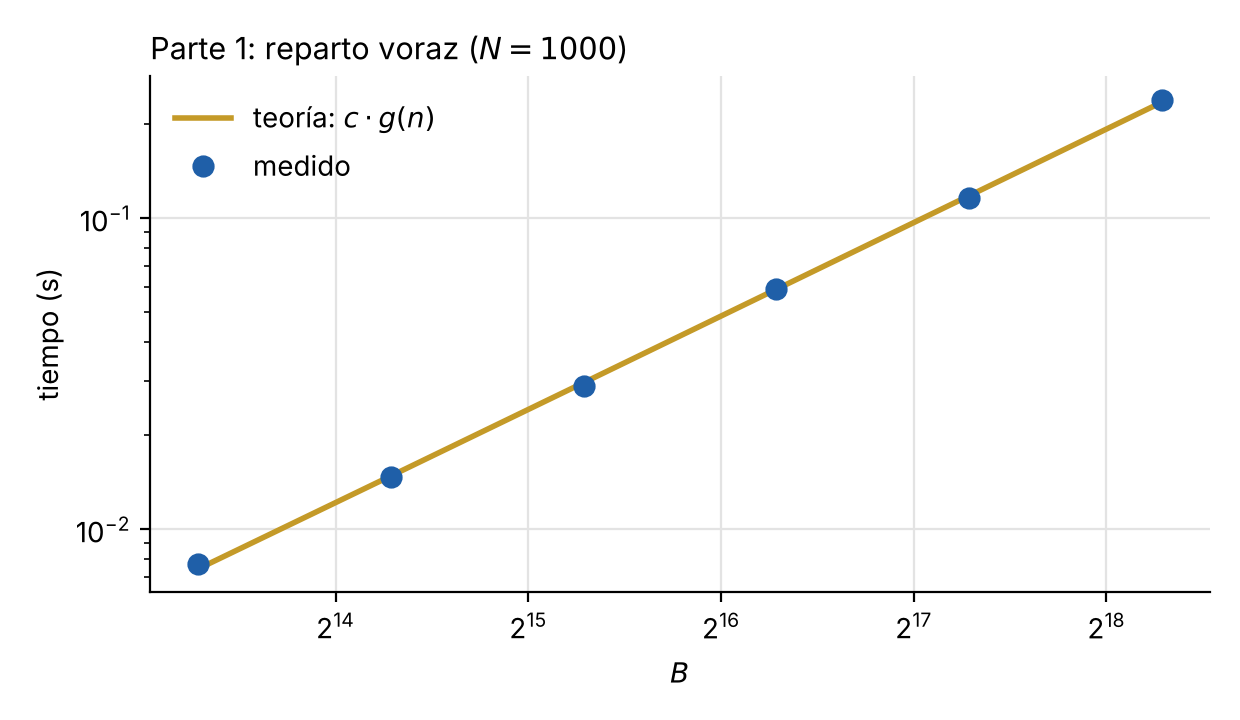
\includegraphics[width=0.49\linewidth]{img/reparto_B.png}\hfill
% 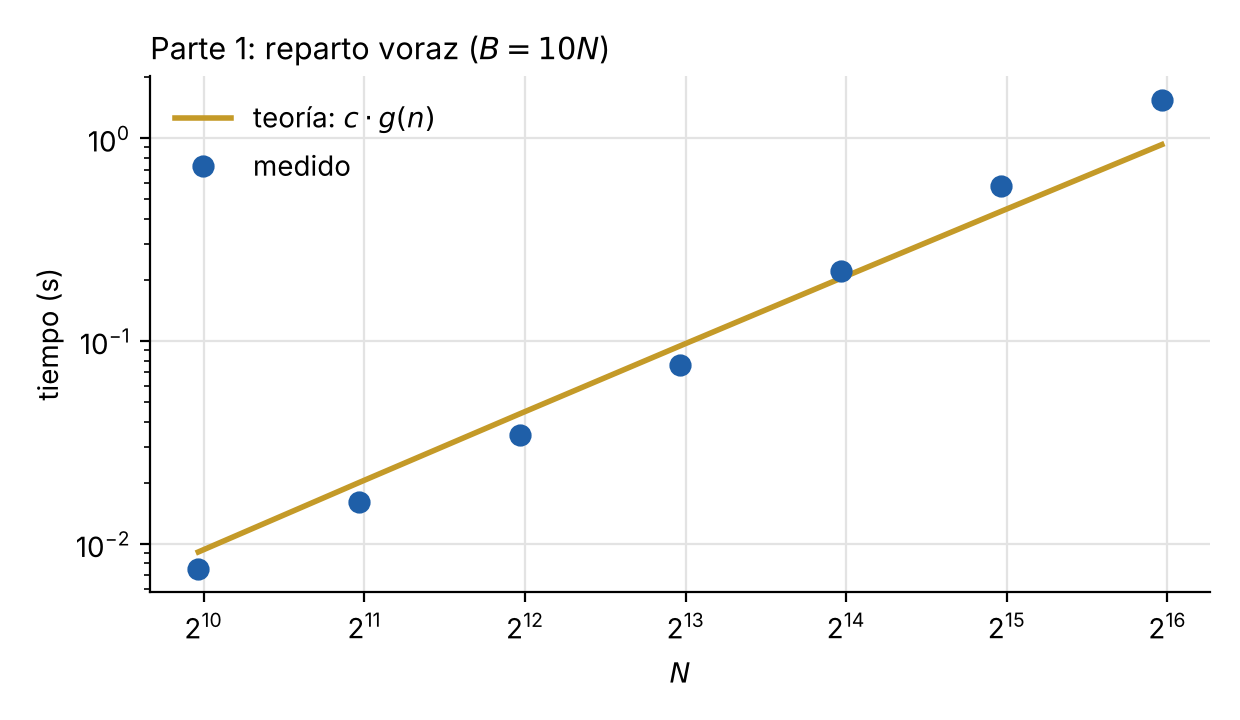
\includegraphics[width=0.49\linewidth]{img/reparto_N.png}
% \caption{Parte 1: tiempo medido (puntos) frente a $c\cdot(N+B\log_2 N)$ (línea), en escala log--log.}
% \label{fig:reparto}
% \end{figure}

% \paragraph{Análisis.} Con $N$ fijo, el cociente $r$ se mantiene en $(7.2$--$7.7)\times10^{-8}$ y la pendiente log--log es 0.99: el tiempo es \textbf{lineal en $B$}, como predice el término $B\log N$. Con $B=10N$, el cociente es estable hasta $N=8000$ y luego crece hasta duplicarse en $N=64\,000$. La causa no es el algoritmo sino la memoria: el análisis supone el modelo RAM, en el que todo acceso cuesta lo mismo, pero cuando el montículo deja de caber en la memoria caché del procesador, cada acceso de \textsc{Extraer-Máximo} e \textsc{Insertar} se vuelve más lento. El crecimiento observado sigue siendo cercano a $N\log N$ (un factor $206$ al multiplicar $N$ por $64$, frente a $102$ predicho, con el factor 2 explicado por la caché) y está muy lejos de un crecimiento cuadrático, que daría un factor $4096$.

% %% ---------------------------------------------------------------------
% \subsection{Parte 2: selección voraz}

% Universo $|U|=1000$ y $|S_j|\in[10,30]$, de modo que $\tau=O(s)$ con $s\le 30$ constante. La columna ``evaluaciones'' cuenta las ganancias $\Delta_j(A)$ calculadas por el programa, y coincide exactamente con la fórmula $kN-k(k-1)/2$ de la Sección~\ref{sec:voraz}.

% \begin{table}[H]
% \centering
% \caption{Selección voraz con $k=20$ fijo. Teoría: $g=kN-k(k-1)/2$.}
% \begin{tabular}{rrrrr}
% \toprule
% \rowcolor{uccielo} $N$ & $k$ & evaluaciones & $T_{\text{medido}}$ (ms) & $r=T/g$ \\
% \midrule
% 500 & 20 & 9\,810 & 11.7 & $1.19\times10^{-6}$ \\
% 1\,000 & 20 & 19\,810 & 24.2 & $1.22\times10^{-6}$ \\
% 2\,000 & 20 & 39\,810 & 53.5 & $1.34\times10^{-6}$ \\
% 4\,000 & 20 & 79\,810 & 104.2 & $1.31\times10^{-6}$ \\
% 8\,000 & 20 & 159\,810 & 209.0 & $1.31\times10^{-6}$ \\
% 16\,000 & 20 & 319\,810 & 416.9 & $1.30\times10^{-6}$ \\
% \bottomrule
% \end{tabular}
% \end{table}

% \begin{table}[H]
% \centering
% \caption{Selección voraz con $N=2000$ fijo. Teoría: $g=kN-k(k-1)/2$.}
% \begin{tabular}{rrrrr}
% \toprule
% \rowcolor{uccielo} $N$ & $k$ & evaluaciones & $T_{\text{medido}}$ (ms) & $r=T/g$ \\
% \midrule
% 2\,000 & 10 & 19\,955 & 27.2 & $1.37\times10^{-6}$ \\
% 2\,000 & 20 & 39\,810 & 51.4 & $1.29\times10^{-6}$ \\
% 2\,000 & 40 & 79\,220 & 84.2 & $1.06\times10^{-6}$ \\
% 2\,000 & 80 & 156\,840 & 141.3 & $9.01\times10^{-7}$ \\
% 2\,000 & 160 & 307\,280 & 248.9 & $8.10\times10^{-7}$ \\
% 2\,000 & 320 & 588\,960 & 462.7 & $7.86\times10^{-7}$ \\
% \bottomrule
% \end{tabular}
% \end{table}

% \begin{figure}[H]
% \centering
% 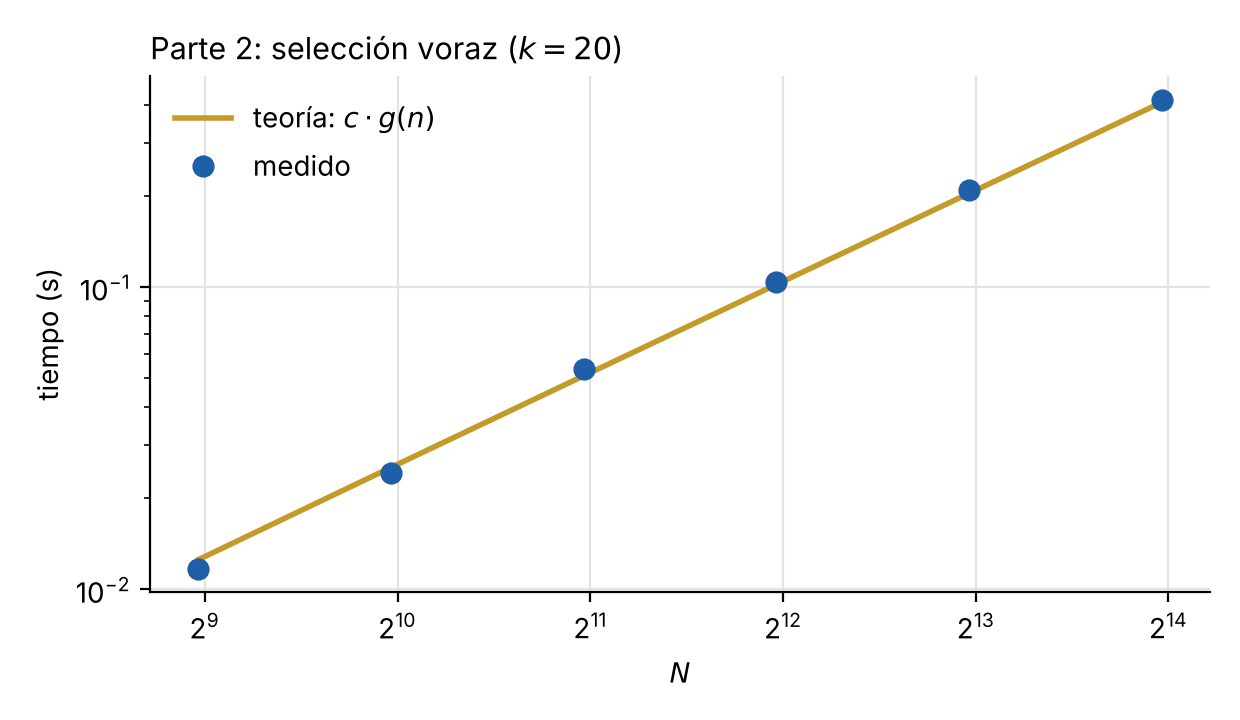
\includegraphics[width=0.49\linewidth]{img/voraz_N.png}\hfill
% 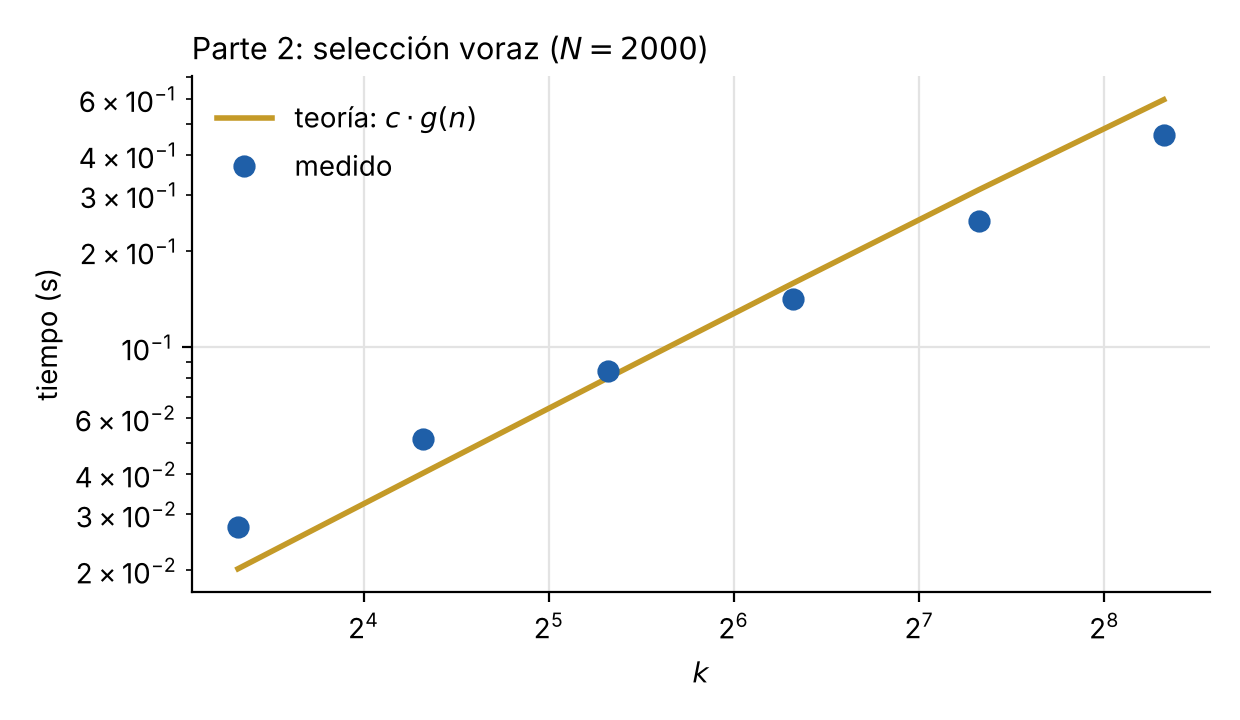
\includegraphics[width=0.49\linewidth]{img/voraz_k.png}
% \caption{Selección voraz: tiempo medido frente a $c\cdot(kN-k(k-1)/2)$, en escala log--log.}
% \label{fig:voraz}
% \end{figure}

% \paragraph{Análisis.} Con $k$ fijo, $r$ es prácticamente constante ($\approx1.3\times10^{-6}$\,s por evaluación) y la pendiente log--log es 1.03: el tiempo es \textbf{lineal en $N$}. Con $N$ fijo, la pendiente es 0.82, algo menor que 1, y $r$ baja de $1.4$ a $0.8\times10^{-6}$. La razón es que $\tau=O(s)$ es una cota superior: cuando $k$ es grande casi todas las categorías ya están cubiertas, y calcular $S_j\setminus C(A)$ produce conjuntos pequeños, que son más baratos de construir. El número de evaluaciones sí sigue exactamente $\Theta(Nk)$.

% %% ---------------------------------------------------------------------
% \subsection{Parte 2: selección exacta}

% Instancias con $|U|=60$, $|S_j|\in[3,8]$ y $k=N/2$, el caso más costoso (Lema~\ref{lem:binom}). Cada hoja calcula $f$ desde cero con $\tau=O(k\,s)$, así que se compara contra $g=\binom{N}{k}\cdot k$.

% \begin{table}[H]
% \centering
% \caption{Selección exacta con $k=N/2$. Teoría: $\binom{N}{k}$ evaluaciones; $g=\binom{N}{k}\,k$.}
% \begin{tabular}{rrrrrr}
% \toprule
% \rowcolor{uccielo} $N$ & $k$ & $\binom{N}{k}$ & evaluaciones & $T_{\text{medido}}$ (ms) & $r=T/g$ \\
% \midrule
% 8 & 4 & 70 & 70 & 0.204 & $7.29\times10^{-7}$ \\
% 10 & 5 & 252 & 252 & 0.458 & $3.63\times10^{-7}$ \\
% 12 & 6 & 924 & 924 & 1.5 & $2.70\times10^{-7}$ \\
% 14 & 7 & 3\,432 & 3\,432 & 5.7 & $2.38\times10^{-7}$ \\
% 16 & 8 & 12\,870 & 12\,870 & 22.6 & $2.20\times10^{-7}$ \\
% 18 & 9 & 48\,620 & 48\,620 & 96.2 & $2.20\times10^{-7}$ \\
% 20 & 10 & 184\,756 & 184\,756 & 371.8 & $2.01\times10^{-7}$ \\
% \bottomrule
% \end{tabular}
% \end{table}

% \begin{figure}[H]
% \centering
% 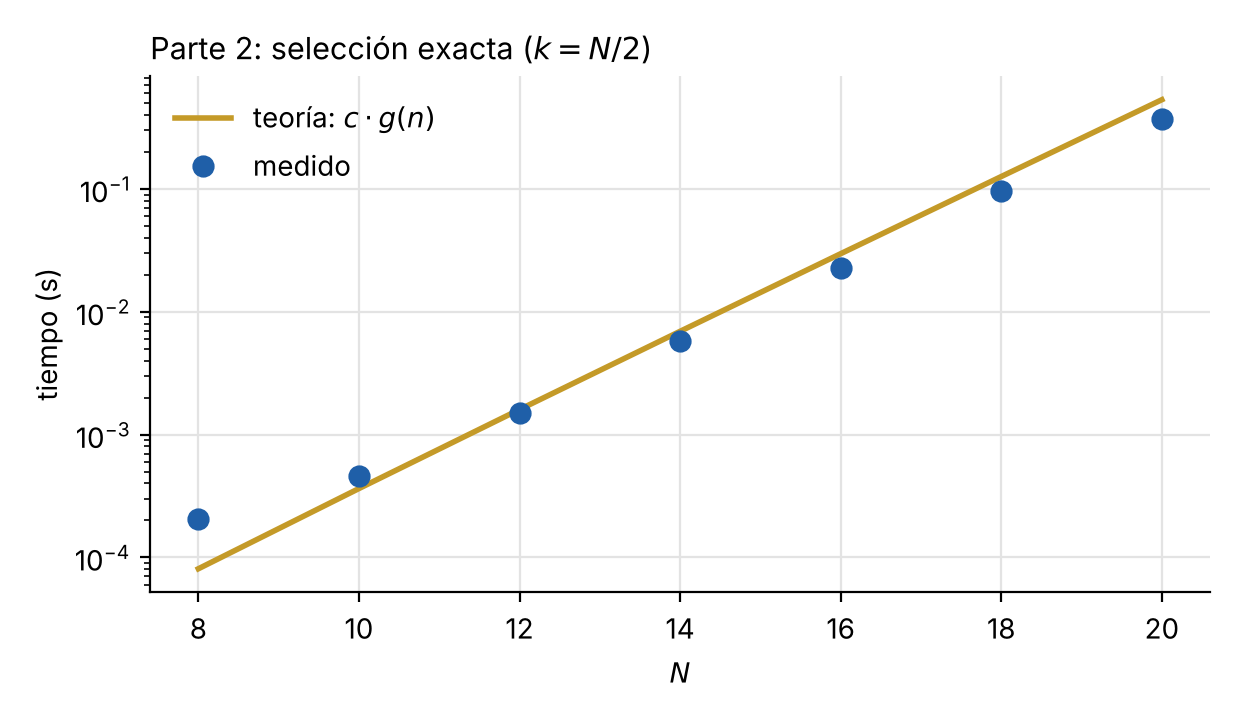
\includegraphics[width=0.6\linewidth]{img/exacto.png}
% \caption{Selección exacta: tiempo medido frente a $c\cdot\binom{N}{N/2}\frac{N}{2}$ (escala semilogarítmica).}
% \label{fig:exacto}
% \end{figure}

% \paragraph{Análisis.} El número de evaluaciones medido es \textbf{exactamente} $\binom{N}{k}$ en todos los casos, como predice la recurrencia de Pascal. En escala semilogarítmica los puntos forman casi una recta: cada vez que $N$ aumenta en 2, el tiempo se multiplica aproximadamente por 4, es decir, crece como $2^N$. Pasar de $N=8$ a $N=20$ multiplica el tiempo por más de $1800$. El cociente $r$ es mayor para $N$ pequeño, donde dominan los costos fijos de las llamadas recursivas, y se estabiliza en $\approx2.2\times10^{-7}$ a partir de $N=14$. Extrapolando, $N=40$ con $k=20$ requeriría $\binom{40}{20}\approx1.4\times10^{11}$ evaluaciones, varios días de cómputo, mientras que el voraz resuelve $N=16\,000$ en menos de medio segundo.

% %% ---------------------------------------------------------------------
% \subsection{Parte 2: verificación de la cota \texorpdfstring{$(1-1/e)$}{(1-1/e)}}

% Como pide el enunciado, la cota del Teorema~\ref{teo:nwf} se verificó calculando el óptimo por fuerza bruta. Para cada configuración $(N,k)$ se generaron 100 instancias con $|U|=25$ y $|S_j|\in[2,7]$, y se calculó la razón $f(A_g)/f(A^*)$.

% \begin{table}[H]
% \centering
% \caption{Razón entre la utilidad del voraz y la óptima (100 instancias por fila).}
% \begin{tabular}{rrrrrr}
% \toprule
% \rowcolor{uccielo} $N$ & $k$ & instancias & razón mínima & razón media & veces óptimo \\
% \midrule
% 10 & 3 & 100 & 0.875 & 0.984 & 80 \\
% 12 & 4 & 100 & 0.895 & 0.985 & 76 \\
% 14 & 5 & 100 & 0.905 & 0.986 & 71 \\
% 16 & 6 & 100 & 0.909 & 0.985 & 71 \\
% 18 & 6 & 100 & 0.913 & 0.979 & 62 \\
% \bottomrule
% \end{tabular}
% \end{table}

% \begin{figure}[H]
% \centering
% 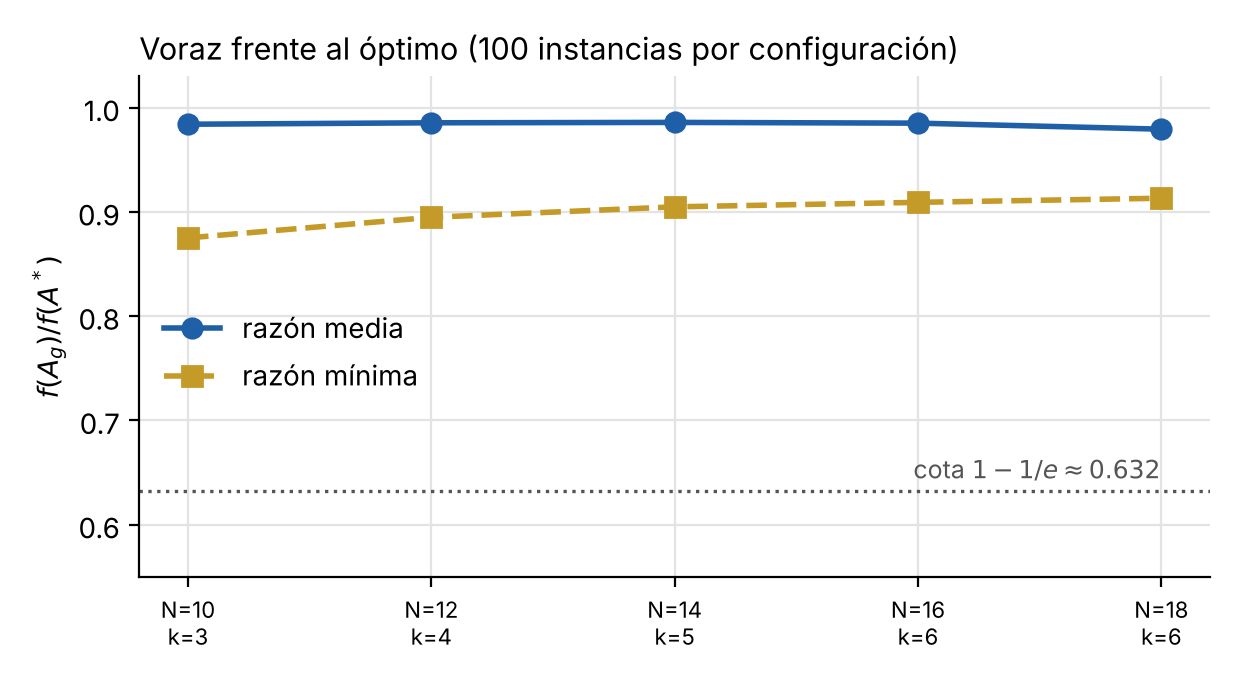
\includegraphics[width=0.65\linewidth]{img/razon.png}
% \caption{Razón media y mínima frente a la cota $1-1/e$.}
% \label{fig:razon}
% \end{figure}

% \paragraph{Análisis.} En las 500 instancias la razón fue siempre mayor que $1-1/e\approx0.632$; la peor fue $0.875$. La cota se cumple con amplio margen: es una garantía para el peor caso posible, y las instancias aleatorias están lejos de ese peor caso. El voraz no siempre es óptimo: falló entre el 20\,\% y el 38\,\% de las veces, lo cual es consistente con la NP-dureza. Un ejemplo pequeño donde falla es $S_1=\{1,2,3,4\}$, $S_2=\{1,2,5\}$, $S_3=\{3,4,6\}$ con $k=2$: el voraz elige $S_1$ primero y obtiene $5$, mientras que el óptimo $\{S_2,S_3\}$ cubre $6$ (razón $5/6$).
% }

\newpage
\section{Conclusiones}

\begin{itemize}
  \item El \textbf{reparto del presupuesto} entre nodos con utilidades cóncavas se resuelve de forma exacta con un algoritmo voraz, cuya optimalidad se demuestra por intercambio. Su función de eficiencia es $\Theta(N+B\log N)$ en el peor caso y $\Theta(N+B)$ en el mejor caso. Es polinomial en $N$ y en el valor de $B$, es decir, pseudo-polinomial; el método del umbral, y la nivelación en el caso continuo, eliminan la dependencia en $B$.
  \item La \textbf{selección de participantes} con utilidad submodular es \textbf{NP-difícil}. Se demostró con la reducción $\MC\le_p\SEL$: cada conjunto se convierte en un nodo y la utilidad es el tamaño de la unión; la transformación es lineal y conserva la respuesta en ambas direcciones.
  \item El algoritmo exacto de la selección realiza $\Theta\big(\binom{N}{k}\big)$ evaluaciones de $f$, con $\tau=O(k\,s)$ cada una; sin cupo, su recurrencia $T(n)=2T(n-1)+c$ da $\Theta(2^N)$. Para $k=\floor{N/2}$ el costo es $\Omega(2^N/N)$, exponencial.
  \item El algoritmo voraz de selección cuesta $\Theta(N\,k)$ evaluaciones, con $\tau=O(s)$ cada una, y garantiza al menos $(1-1/e)\approx 63\%$ del óptimo \parencite{nemhauser1978}; esta garantía es la mejor alcanzable en tiempo polinomial a menos que $\mathrm{P}=\mathrm{NP}$ \parencite{feige1998}.
  \item Como la selección es un caso particular del problema completo del proyecto, la dificultad del proyecto se concentra en elegir los participantes, no en repartir el presupuesto.
\end{itemize}

\paragraph{Trabajo pendiente.} Este informe cubre la solución base de las dos partes. Las variantes obligatorias (costos de participación, repetición en $T$ rondas con fallas y nodos relacionados entre sí) se desarrollarán en la siguiente entrega. Para la variante con costos, la cota del voraz cambia y debe citarse en su versión para cobertura con presupuesto \parencite{khuller1999}.


\newpage
\appendix
\section{Código de los algoritmos}\label{anexo:codigo}
El código completo, incluido el generador de instancias y las mediciones (\texttt{code/experimentos.py}), acompaña este informe. Para reproducir las tablas y gráficas de la Sección~\ref{sec:experimentos} basta ejecutar \texttt{python code/experimentos.py} desde la carpeta del informe.
\lstinputlisting[language=Python]{code/algoritmos.py}

\newpage
\printbibliography[title={Referencias}]
\end{document}
